\documentclass[12pt,a4paper,notitlepage,twocolumn]{report}
\usepackage{epsfig,graphics,subfigure}
\usepackage[a4paper]{geometry} \usepackage[final]{pdfpages}
\geometry{top=0.5in, left= 1.0in, right = 1.0in} \author{*} \title{*}
\date{}
\begin{document}
%\maketitle

\widowpenalty=5000

\section*{Overview}
The objective of the System Design Project (SDP) was to build a robot
that can play Robocup-like soccer competitively using a 10-person
team. The first probleim faced in SDP is to come up with a way to
efficiently use the available resources (manpower) and to channel the
development effort so as to prevent duplication of effort as well as
minimising the interdependencies between the sub-systems to reduce the
communication costs.

\section*{System Architecture}
Though our initial design and system architecture slowly evolved over
time, there were no dramatic differences between the first and the
final architecture of our system. We decided to first posit a number
of sub-systems and high-level interfaces between them. Doing this
helped organise our overall development effort. The final system
architecture is illustrated in Figure~\ref{fig:arch}.

\begin{figure} [ht]
  \centering
  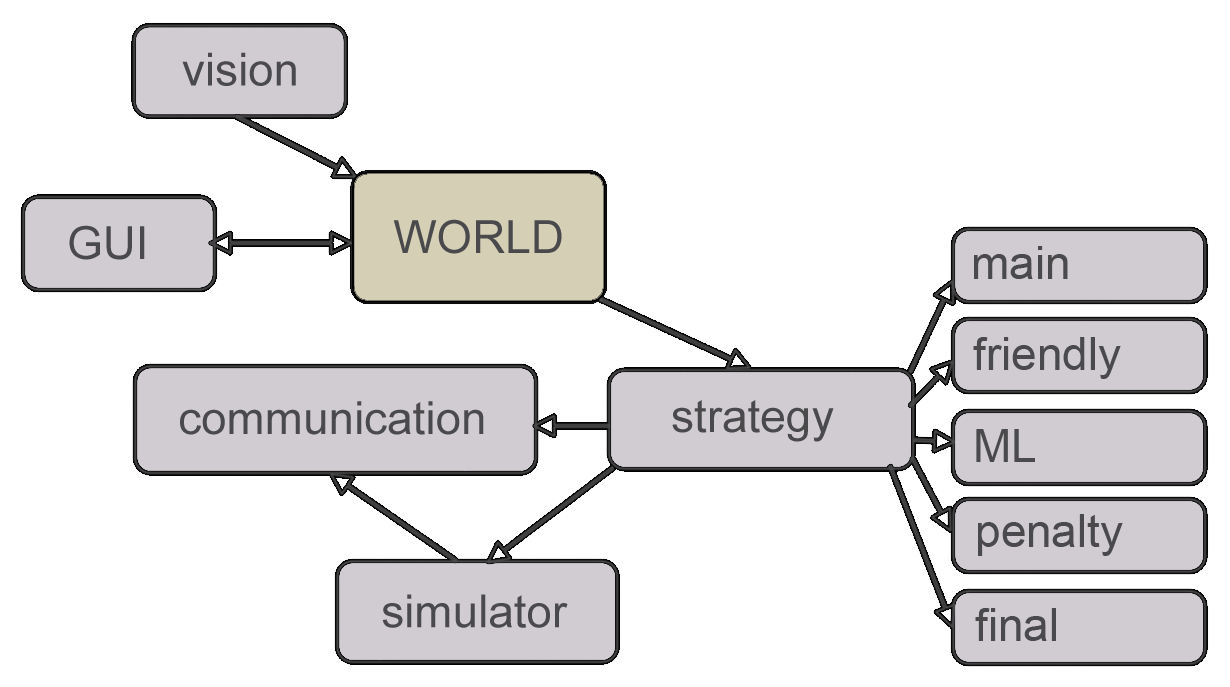
\includegraphics[width=70mm]{arch.png}
  \caption{The system architecture and the information flow between
    the various sub-systems. The links from the strategy sub-system
    are examples of the different strategies that the system could be
    instructed to run. Not shown are the vision-camera links and the
    communication server - robot links.}
  \label{fig:arch}
\end{figure}

\section*{Management and Organisation}

After looking at past SDP projects to get a flavour of how they
managed the team we initially decided not to use a specific management
technique but rather adopt a more democratic approach. The team was
split in line with our outlined architecture, i.e., into groups
focused on robotics, vision, communication, and strategy,
respectively. This assignment was done based on individual preference
and most of the decision making was left to the respective subgroups.

 The more relaxed approach seemed to be going very well up until the
poor performance during the first milestone. After the subsequent
meeting with the team, it was clear that most individuals were not
aware of how other subgroups were progressing and that more emphasis
towards integration testing was needed. The frequent meetings were a
key reason for subsequently choosing SCRUM over other methodologies.
Although meeting everyday was sometimes not practical, we tried to
ensure that everyone, be it as a whole group or a subgroup, met at
least three times a week. Further to this, each member had a
development diary which they would use to document their work and
allow any people who missed the meeting to keep up to date with our
progress. The added formality of SCRUM greatly improved the efficiency
of our work.In particular, the use of pair programming meant that the
less experienced programmers in our group could be paired with someone
who could more readily translate their ideas into code.

\subsection*{Planning and Progress}
The progress management broke down into two key aspects: What had to
be done, and what would happen if we didn't do it.

The first step was to create a Google Docs spreadsheet. which
contained information about what had to be done, how important is was,
its current status, and who was carrying it out. These tasks were
assigned and discussed during our regular SCRUM meet ups.

The second step was to consider the risks involved with certain tasks.
We used a risk management chart (Figure~\ref{fig:riskman}) for this with the
aim being to classify each potential stumbling block based on
likelihood against severity of occurrence. This helped us to ensure
that any tasks in the red were handled immediately and with due care.

% \begin{figure*} [ht]
%   \centering
%   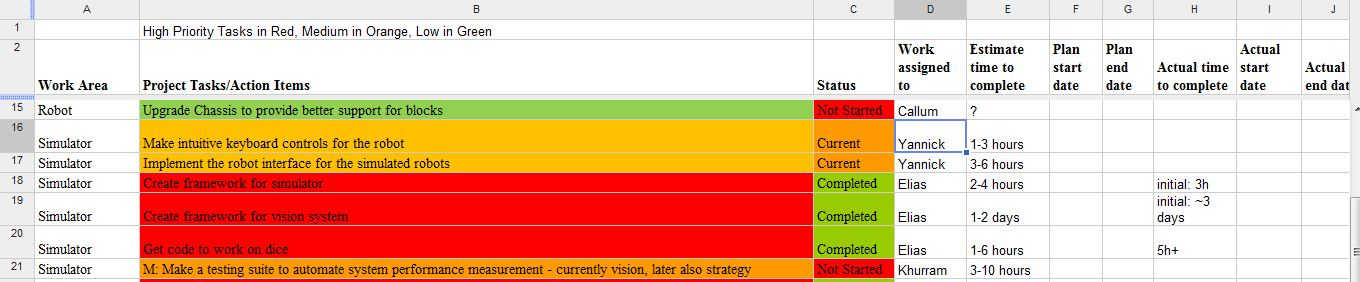
\includegraphics[width=150mm]{designc.jpg}
%   \caption{Design Capture}
%   \label{fig:designc}
% \end{figure*}

\begin{figure*} [ht]
  \centering
  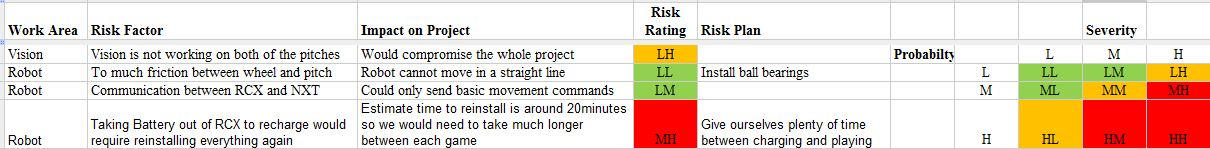
\includegraphics[width=150mm]{riskman.jpg}
  \caption{Risk Management}
  \label{fig:riskman}
\end{figure*}



\section*{Robot Design}
When it came to the design of the robot it was decided that we would
aim to create an innovative design with the aim of improving on the
efforts of previous robots.

Looking at designs from the previous years of the course we realised
that the best robots:
\begin{enumerate}
\item were {\em manoeuvrable}, allowing for quick and direct movement
  to the ball,
\item had {\em strong kickers} to allow for powerful kicks right
  across the pitch and off the side walls,
\item were built with {\em strong chassis} to put up with aggressive
  game play, and
\item were {\em simple} , making it easy to write their control system
  software.
\end{enumerate}
Of these key areas, we decided to focus on manoeuvrability and
strength, deeming them the most important.

The last years’ recorded games indicated that much time was wasted by
the need for many robots to stop and turn before they could move to
the ball. A design that could move to the ball directly would have a
big advantage against these “traditional” robots.

Having established the need for an agile and manoeuvrable robot, we
needed to find a suitable wheel design. The majority of past designs
made use of two conventional static wheels placed on either side of
the robot's chassis; the wheels would be individually powered in order
to move and turn the robot.
\subsection*{The Traditional Wheels}
\textbf{Static wheels} are conceptually simple, reliable and cheaply
implemented using the standard Lego NXT kit. For all their advantages,
static wheels don’t allow for direct movement to the ball in general,
since the robot has to be either stopped and turned or turned by
moving the wheels on different sides by differing amounts.

 In addition to the challenges with steering, in order to maximise the
manoeuvrability that can be achieved using static wheels very large
wheels were required to reduce the overhangs at the front and the rear
of the chassis. Larger wheels reduced chassis space and this would
make it harder to fit in a powerful kicker design.\newline

\textbf{Tank-Style caterpillar tracks} offer another way to eliminate
the problems associated with big wheels. As well as reducing the space
required for large wheels, they could in theory also provide better
grip on rough surfaces due to the increased surface area in contact
with the ground.

 However, contrary to past years, this year’s painted pitch
surface is very smooth, and consequently many groups experienced
problems with grip using caterpillar tracks, which made tank tracks
unsuitable for a high-performance design.

Besides the grip issues associated with caterpillar tracks, a robot
fitted with them still had to stop and turn in order to move to a
direction perpendicular to it. This limited their potential for
manoeuvrability of a track-equipped robot similar to one with static
wheels.\newline

\textbf{Omni wheels} were the solution chosen by the 2010 winning team
in order to maximise manoeuvrability and to get around the need for
having to stop and turn. Omni wheels are holonomic, allowing direct
movement in any direction. The omni wheels are made up of a set of
rollers positioned around the circumference of the wheel, allowing for
movement that is perpendicular to the wheel's axis of rotation.

By using four powered omni wheels, the 2010 wining team created a
robot platform which could move in any direction without turning while
still allowing their robot to rotate around it's own axis. Although
these wheels seemed very appealing for maximising the manoeuvrability
of our robot, they had some drawbacks:

\begin{enumerate}
\item Omni wheels are complex and many pre-2010 groups struggled to make their robots move with them,
\item the wheels give little grip since the rollers have little surface contact overall,
\item omni wheels are a specialist product that have to be ordered from abroad at high cost, and
\item the shipping of the omni wheels would have taken fairly long..
\end{enumerate}
With these disadvantages in mind, we felt that omni wheels were not
the ideal solution for flexible movement.

\subsection*{Our Novel Wheel Design}

\begin{figure} [ht]
  \centering
  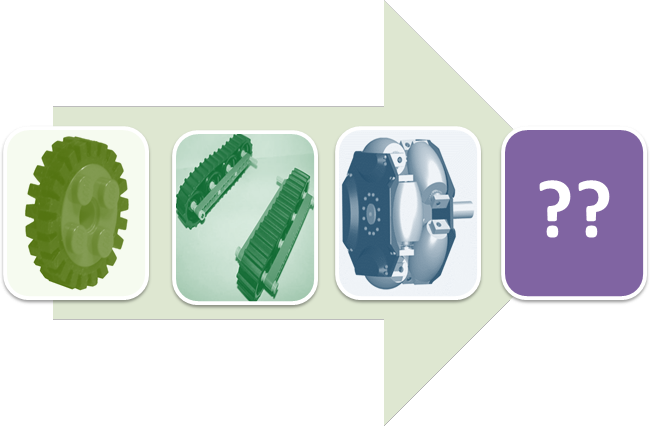
\includegraphics[width=60mm]{wheels.png}
  \label{fig:turntable}
\end{figure}

After considering the wheel types used by previous robots we came up
with a novel design we call the \textbf{turntable wheel}. Using a Lego
turntable provided in our NXT kit, we could make a conventional static
wheel which could be independently turned and powered to permit
movement in any direction. The turntables allow for this by providing
a movable platform with a central opening through which drive
components could be fed from one side of the component to the other.

The turntable wheels can be seen as a fusion between the static wheels
and {\em holonomic} wheels: the turntable wheels provide the
conceptual simplicity and the levels of grip of the static wheels
while also giving high levels of manoeuvrability as provided by the
holonomic designs. We decided that the risk of using this untested
technology was more than outweighed by the potential advantage this
design could offer in terms of manoeuvrability while avoiding the grip
issues, the complexity, and the costs associated with the holonomic
wheels.

\begin{figure} [ht]
  \centering
  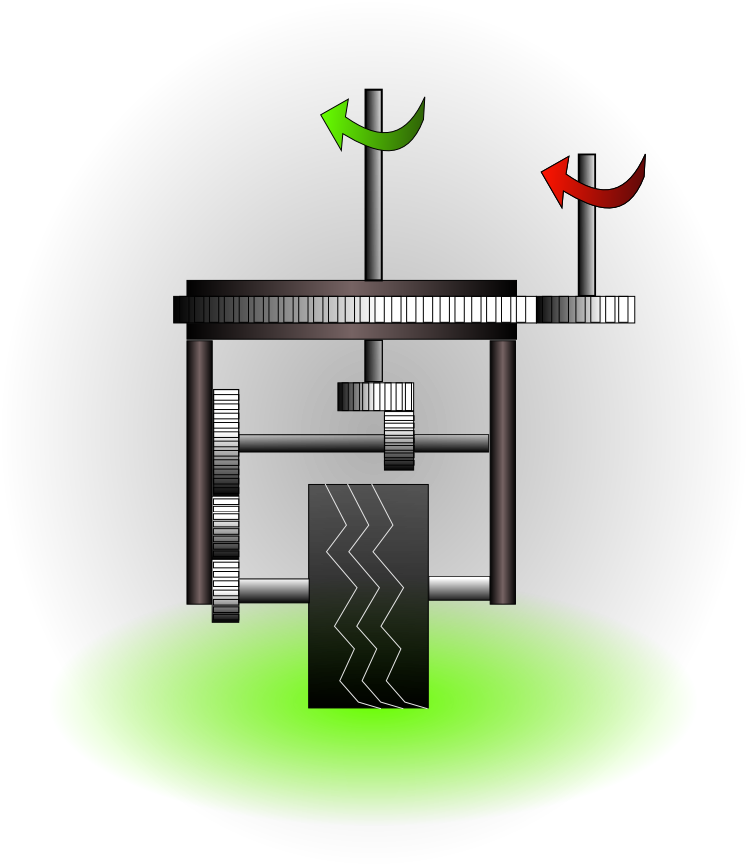
\includegraphics[width=60mm]{turntable.png}
  \label{fig:turntable}
  \caption{The turntable wheel}
\end{figure}

\subsection*{Chassis}
Having decided on the turntable wheels, we created a chassis in which
they could be effectively utilised. The chassis of our robot houses
two turntable wheels placed in opposite corners with ball bearings on
the remaining two corners to balance the robot.

\begin{figure} [ht]
  \centering
  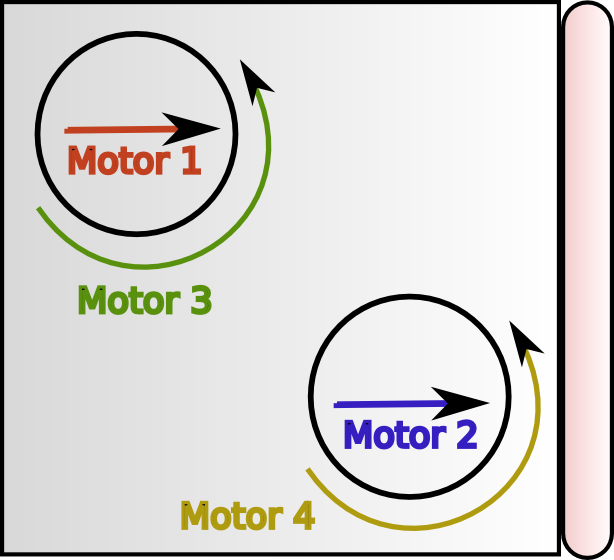
\includegraphics[width=45mm]{chassis.png}
  \label{fig:chassis}
  \caption{Chassis Design}
\end{figure}

In total, our design used 5 motors, 4 for the two turntable wheels,
and an extra motor to power the robot’s kicker. Since the NXT control
brick could only support 3 motors, it was necessary to use a motor
multiplexer board to drive the extra motors.

\section*{Vision}
The function of the vision system is to take as input the raw camera
input and to produce as output the position of the ball as well as the
position and the orientation or the bearing of the two robots on the
pitch. The vision system’s responsibilities are limited to what it can
extract from a single image, disregarding any previous images. That
is, the vision system is stateless, and can be considered to produce
intermediate-level features from low-level features (the unprocessed
camera input).

To add to conceptual clarity, and to minimise duplication of effort in
creating high-level representations of the pitch state, we created an
intermediary sub-system called the “world” to bridge the stateless
vision system and the strategy systems together. Without this
sub-system, each piece of strategy code would have potentially needed
to implement their own ways to create the higher-level visual
features. An added benefit of this split is that, irrespective of the
strategy component used, each of the useful high-level features can be
uniformly visualised with the vision GUI (and thus also eliminating
any dependency between the strategy components and the GUI).

Our vision system implementation uses OpenCV with Python to achieve
good performance and to be fairly flexible. Our complete system
processes slightly more than 25 frames per second on the allocated
DICE machines, beating the frame rate of the pitch camera.

The vision system is split into the following three logically distinct
components:

{\em Image acquisition}: initially we used the native OpenCV methods
for this, but eventually found that MPlayer worked better since some
of the DICE machines started to mysteriously fail with the OpenCV
methods.

{\em Preprocessing}: the frame is cropped and undistorted (though
ultimately we disabled undistortion since we failed to get good camera
calibration data).

{\em Feature extraction}: the objects in the image are recognised
using a combination of thresholding and an iterative method for
estimating the orientation. We spent tons of time trying to get this
right and finally succeeded in making the vision system very robust
and capable of detecting the objects in virtually all situations where
it mattered.

\subsection*{Feature extraction explained}
After trying out a lot of different methods, we finally managed to
reduce the vision system to a simple core that performs very well
under virtually all real-world match situations. The resulting vision
system is perhaps deceptively simple in hindsight, but the problem is
in finding the right simple methods for making it work.

A key aspect to our ultimately well-performing vision system is that
the threshold calibration is very easy and fast to do with the system
GUI (the threshold calibration sliders for each threshold can be
toggled with a key press). Prior to doing this, we spent a lot of time
manually adjusting the threshold constants in the code base, without
too much success.

Our system uses thresholding as its basic filtering mechanism using
well-calibrated thresholds, usually for each pitch separately (the
lighting conditions vary considerably). There are four basic
thresholds (ranges of colour values in the RGB or the HSV colour
space), one for each of: the ball, the blue T, the yellow T, as well
as the direction marker. Of these, the black direction marker is the
most problematic (since it is nowhere near as dark as it looks), while
the rest of the thresholds almost always give exclusively the right
“object” and nothing else (see Figure~\ref{fig:thresh} for the difference).

To be able to obtain the robot’s direction accurately, we found that
the direction marker is virtually necessary; deriving the direction
using the best-fitting bounding box of the T or the robot’s chassis
can be wrong by up to 40°. To get a better-quality thresholded image
for the direction marker, we initially also included background
subtraction in the preprocessing stage, but ultimately found that we
could not make the background-subtracted intermediate image work in
all the normal situations.

Our ultimate solution to the problem of finding the black direction
marker involves using the shape of the thresholded T by finding the
direction its “top part” is facing by finding its \emph{central
  moment} (or its centre of gravity). Using the central moment and the
centre of the bounding box of the thresholded T, we obtain the
direction of the robot with relatively low accuracy (up to ±40°). We
then proceed to refining this estimate by using bitwise AND over the
pixels of the direction marker-thresholded image, using a
circle-shaped bitmask of increasing radius that is centered near the
expected location of the direction marker (a fixed distance towards
the low-accuracy expected heading of the T). We iterate this process
until we find the AND operation yields a result that is above a fixed
number of pixels (we used ~10 pixels for this). We find that this
method is very accurate, though it sometimes gives wrong results near
the pitch corners (where the correctness usually does not matter at
all anyway).

\begin{figure}[htp]
  \begin{center}
    \subfigure[thresholding for the coloured T]{
      \label{fig:thresh_t}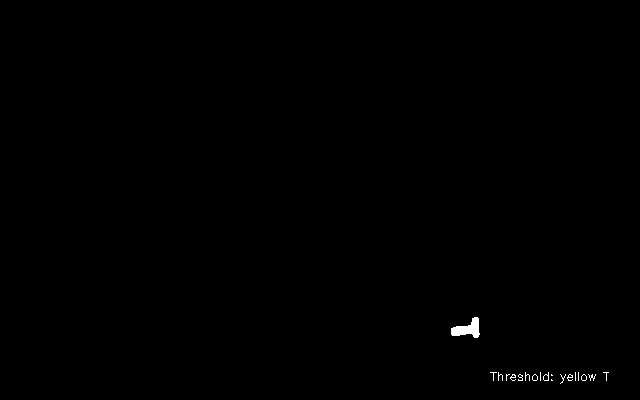
\includegraphics[width=60mm,height=30mm]{thresh_t.jpg}
    }
    \subfigure[thresholding for the direction marker]{
      \label{fig:thresh_marker}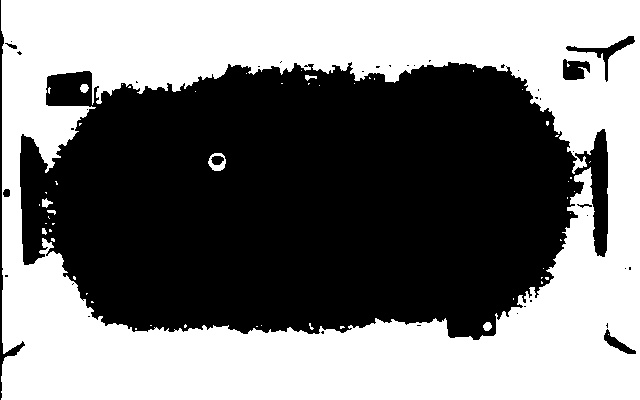
\includegraphics[width=60mm,height=30mm]{thresh_marker.jpg}
    }
  \end{center}
  \caption{The thresholded images}
  \label{fig:thresh}
\end{figure}

\section*{Robot control system}
We programmed the physical robot system in Java, using a custom NXT
firmware called Lejos. We chose Lejos without looking too much into
alternatives as Lejos was easy to use and had a great library
containing virtually all the functions we would need to make the NXT
do anything.

Our initial design of the control system was made to be as “stateless”
as possible, such that raw motor commands would be send and would
remain in effect until a new command overrode them. This, we thought,
would make the robot extremely responsive and capable of reacting to
new circumstances immediately. Though we could send up to 50-70
commands per second second, we found that the camera latency (around
300-400 ms) would cause heavy oscillations since commands were based
on outdated information and consequently the robot would almost always
offshoot the target.

In hindsight, \emph{visual servoing} could have possibly solved this problem
almost perfectly, although the “hidden states” of the turntable wheels
might have made it too complicated. However, we very much recommend
teams with simpler designs to try out a visual servoing solution.

To cope with problematic direct motor commands, we migrated some of
the commands previously used in the PC-side strategy code directly
onto the robot. These commands included: straight-line movement along
some bearing relative to the robot, as well as rotating the robot
along its own axis by a specified angle. The migrated commands would
execute on a longer timescale than with the previous command protocol
(approx. 1 or 2 per second). With the control system, the commands
would take a non-deterministic amount of time to execute, which, as we
found out near the final match, would cause problems with large-scale
“oscillation” related to ignoring most of the received commands and
only executing the latest one.

\subsection*{Communication server}
From the very start, one of the key requirements for our system was to
have a reliable and robust connection with the robot. Since the robot
control system being developed in Java using the Lejos library, we
decided that using the corresponding computer-side communication
classes would ensure a match up in protocols.

Since the rest of our system was written and Python, and in order to
make the communications well-encapsulated part, we opted create a
simple, stable socket server that would initialise a Bluetooth
connection and keep it open as long as possible. The socket server
would then act as a proxy for the strategy system to transmit
commands. Since the communication server would keep the Bluetooth
connection open regardless of the strategy code, we spent less time on
resetting the robot and also gained the ability to switch between
different strategies on the fly.

The first priority for us was to some basic bridge between the robot
and the strategy system. After this was achieved, we focused on making
the sub-system even more robust through the adding of reconnection
features if a connection got closed for some reason, as well as more
capable by adding the ability to receive incoming data from the robot
(sensor inputs).

\section*{Strategy}
At an architectural level, the strategy system is merely an interface
used for handling abstracted robot commands as well as to receive
abstracted vision information from the world module. In the default
mode of operation, the world module would be hooked up to the vision
system and the communication interface would point to the Bluetooth
interface server, but, both were made abstract to permit hooking the
code into simulated equivalents to allow for testing sub-systems
independently.

We built the strategy system in accordance to match our first
communication protocol, such that each strategy module functions by
taking in a world state and outputting a command based on that state
alone, i.e. sending about 25 commands per second. Though the
assumptions we used for deciding on this mode of operation had
changed, we never really considered changing way the strategy system
worked until it was too late.

Since the later robot command protocol executed only 1 or 2 commands
per second, ignoring the rest, the new combined control system could
exhibit much larger-scale “oscillations” where the robot would drive
forward for far too long until a later command was received. These
oscillations were caused by the robot ignoring most of the commands
and only executing the ones that (sometimes) happened to correspond to
more or less what it was doing anyway.

Though we never came up with a satisfactory solutions to these
problems (in time!), should a future SDP team create a robot with
design similar to ours, we strongly advise for designing the
strategy/control system such that commands would get sent when deemed
necessary (for major “course changes”), i.e. that there be some part
that interprets what the system currently does, and decides whether a
change would be beneficial, sending a move to the idle robot control
system. However, this is a complex proposal where much could go wrong.
Something simpler like visual servoing should be tried first. A third
possibility would be to “aggregate” the commands and send the
mean/median command (whatever that means).

\subsection*{Simulator}
Early on we realised we would have many difficulties developing good
ways to control our unconventionally designed robot. Until relatively
late into the course, we would often have various problems with our
physical robot: the design might not have been robust enough, some
component was physically broken, the batteries were out of charge,
etc., so we needed to have an alternate way to test at least some
parts of our system without needing to use the “costly” robot. For
this reason, and since our vision system wasn’t very reliable until
sometime near the first friendly match, we created a simulator that
could accurately duplicate our robot’s physics, to visualise and
otherwise test the performance of different strategies.


\subsection*{Reinforcement learning and artificial potential fields}
Since we expected that the competition in SDP would be much harder
this year, we looked out to see if we could further use some proven
state-of-the-art techniques from actual Robocup tournaments. We found
two promising candidates: \emph{reinforcement learning} and
\emph{artificial potential fields}.

We implemented a basic reinforcement learner system using our
simulator. The learner used an algorithm called \emph{fitted value iteration}
which would first explore various actions given a state of the robot
relative to the ball, and always choose the one that yielded the best
expected reward (defined by the reward function that would essentially
reward kicking the ball correctly and penalise inaction or going the
wrong way). Unfortunately, though the basic approach seemed sound, the
performance of the learning system was far too low to yield usable
results before the end of SDP (the system was written in Python/Numpy
and further compiled using Cython). Though this failure falls under
doing something too complicated in hindsight, we expect that
reimplementing the reinforcement learner and its physics model in C
would have yielded the speedups to make it work (the system would have
needed to be a few orders of magnitude faster).

Artificial potential fields (APFs) have been widely used for many
robot planning tasks. We realised that APFs, properly calibrated,
would make a simple and attractive way to guide our early robot using
direct motor control. APFs are computationally very cheap to use and
compactly specify the direction a robot should move in: towards the
ball in the right away, and around the opposing robot. Though we did
get some promising results using APFs, especially in the simulator,
ultimately we experienced similar problems as we had with the earlier
direct motor control attempts: the robot would move in a jittery way,
and since the robot could not, in general, move while turning, the
speed of the robot would be greatly reduced. Another problem we had
with APFs was that it was difficult to get the shape of the
magnet-like directed potential field surrounding the ball to be
exactly the right shape. In Figure~\ref{fig:apf}, the field is shown to be
slightly too “wide” than would seem optimal. Ultimately we replaced
APF-based movement with straight line movement using virtual landmarks
(as described below).

\begin{figure} [ht]
  \centering
  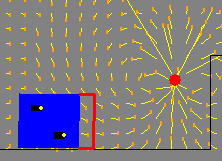
\includegraphics[width=60mm]{apf.png}
  \label{fig:apf}
  \caption{A visualisation of artificial potential fields in the simulator}
\end{figure}

\subsection*{Virtual landmark-based navigation}
\begin{figure} [ht]
  \centering
  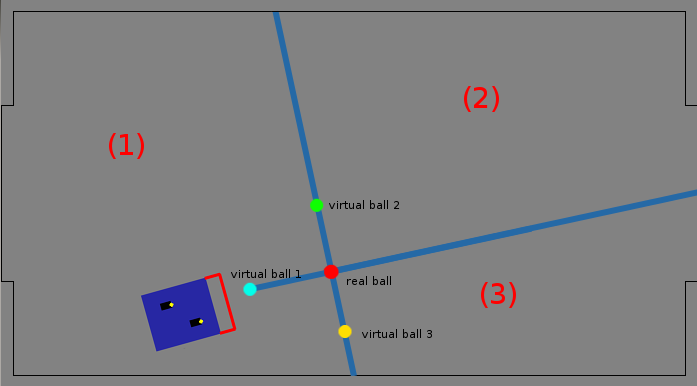
\includegraphics[width=60mm]{vball.png}
  \label{fig:vball}
  \caption{A visualisation of the landmark-based navigation method}
\end{figure}

This was the first method we evaluated for making the robot score
goals. With this method, the robot navigates to virtual landmarks (or
balls) rather than to the actual ball. The virtual balls are placed so
as to assist the robot in kicking the ball “behind” it without first
colliding with it. As can be seen, the landmarks are placed so as to
“point to” the opponent’s goal. The strategy code for using this
method then consists of three rules:
\begin{enumerate}
\item If the robot is between the ball and landmark 1, go to the ball.
\item If the robot is in area (1), move to landmark 1.
\item If the robot is in area (2) or (3), go towards and past the
  closest landmark.
\end{enumerate}

\subsection*{Subsumption architecture and geometric movement planning}
Our final strategy builds on all the previous ones and involves a
somewhat sophisticated set of features used for directing the robot
towards certain “points of interest”. The main feature of this
strategy is the use of “goal-target cone points”. As seen in the
following screenshots of our system GUI, we draw a circle of fixed
distance around the ball and project on it points corresponding to the
“optimal” kicking position for each player, as well as the
corresponding bounds: if the robot is close the opponent’s goal, the
bounds are loose, but otherwise the robot would have to be very
precise its approach angle if it wanted to score a goal with just one
kick. For more detail, see the world/strategy code (it should be
fairly readable).

Ultimately, we implemented this strategy far too late and even had to
disable parts of it while doing the final tests when we found certain
parts of it to be broken or otherwise not behaving as expected. We
ultimately managed to make the core logic into a linear sequence of
if-then rules, classifying the combination of the robot and strategy
as having what’s called the \emph{subsumption architecture}.

Below are the simplified rules for the implied subsumption
architecture rule set (only the first matched rule is executed):
\begin{enumerate}
\item If the ball is far from me and the opponent is near the ball, go
  between the ball and my goal.
\item If the ball is far from me and the opponent is not near the
  ball, go towards the goal-kick point (the thick blue/yellow point on
  the circle matching the robot colour).
\item If my approach angle to the ball is within the bounds (smaller
  circles), go to the ball directly.
\item If I am not between the ball and my goal, go to the nearest
  tangent (the barely visible circles).
\item If the opponent is near the ball, go between the ball and my
  goal (play defensive).
\item If I am near the opponent’s goal (the ball is guaranteed to be
  near now), move to the goal-kick point.
\item If nothing else applies, go directly to the ball.
\end{enumerate}

\section*{System GUI}

\begin{figure*}[htp]
  \begin{center}
    \subfigure{
      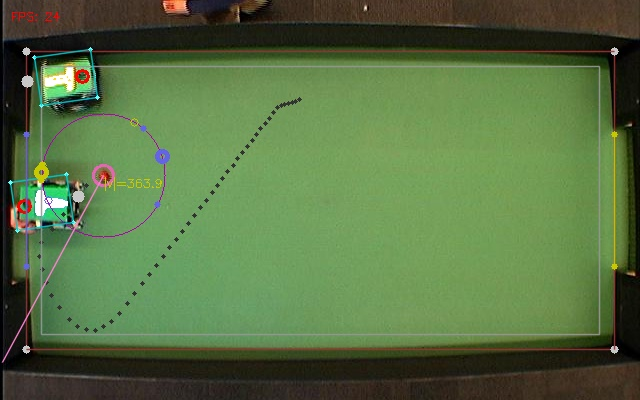
\includegraphics[width=75mm]{gui1.jpg}
    }
    \subfigure{
      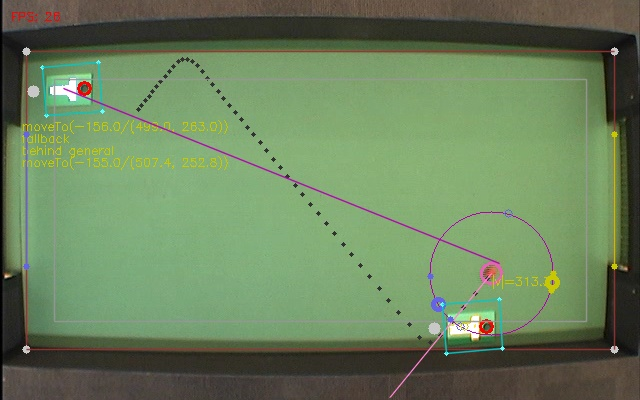
\includegraphics[width=75mm]{gui2.jpg}
    }
    \subfigure{
      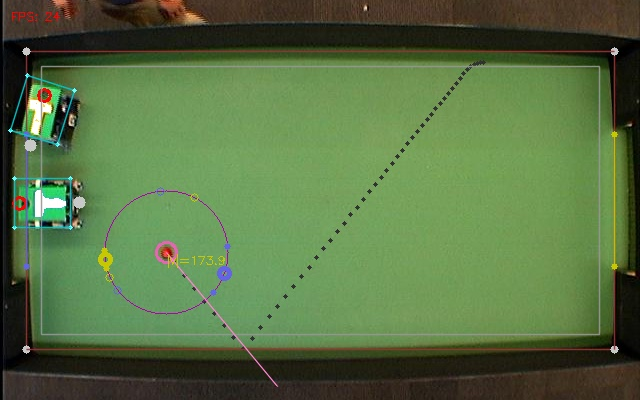
\includegraphics[width=75mm]{gui3.jpg}
    }
    \subfigure{
      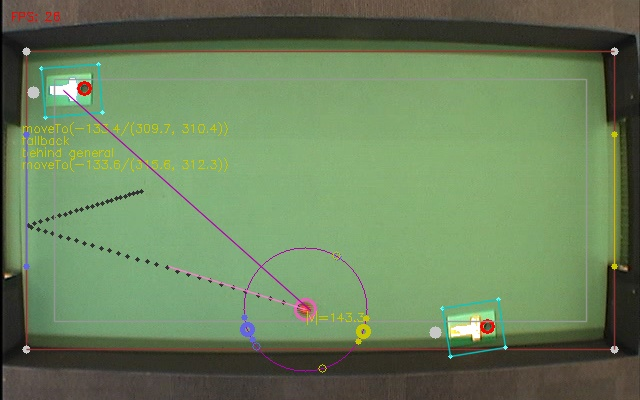
\includegraphics[width=75mm]{gui4.jpg}
    }
  \end{center}
  \caption{\emph{Don’t} handle special cases where possible; in this
    case, the apparent erroneous trajectory prediction adds
    robustness: the pitch geometry tends to produce similar effects,
    and the opposing robot might block the ball anyway. We get
    contingency-handling for free using the simplified trajectory.}
  \label{fig:gui}
\end{figure*}

We designed the system GUI to be minimalist and yet to show all
relevant intermediate and high-level features on the screen by
default, as well as providing keyboard controls for hiding everything.
The system GUI is associated with the strategy and robot side/colour
selector (not shown) which allows for picking any combination of the
three on the fly. See Figure~\ref{fig:gui} for screenshots of our
system GUI.

\section*{World}
The function of the world is to take as input the positions and
orientations of each object on the pitch from the vision sub-system
and to produce as output various high-level features based on them.
The high-level features coded in were created one by one when some
strategy component was found to have use for them. Being true to the
system architecture diagram, as shown in the system GUI above, the
world is agnostic of the side of the robot, making the world subsystem
well-encapsulated and simple to work with. The high-level features
provided by the world subsystem include:

\begin{itemize}
\item Ball and robot velocity vectors
\item The boundaries of the pitch and the positions of each goal
\item Estimated ball trajectories indexed by time (up to 5 seconds
  into the future, in 100 ms increments)
\item “Goal-target cones” for estimating when the ball would hit the
  goal if kicked
\item Approximate bounding boxes of the robots for collision avoidance
  in the strategy code
\end{itemize}

\section*{Evaluation and future extensions}

Our team came up with a unique design that no team had used before.
The challenges were great and we were unfortunately unable to deliver
in the final matches. However, with some refinement, we believe that
the turntable wheels have the potential to be a winning design and so
hope that any future SDP students who read our documentation can learn
from our mistakes and get the best out of such an interesting design.

In the final match, our robot would take unexpectedly long to switch
between different commands. This led to the sort of oscillating
behaviour we described in the section dealing with the control system,
and consequently our robot lost the match against a similarly low
performance robot with 0-1 score.

\subsection*{Recommendations for component reuse}
\begin{itemize}
\item We recommend using our vision system and the associated world
  module. Probably the only remaining enhancement for the vision
  system would be to add the correct camera calibration data to remove
  the barrel distortion. The world module requires some audit
  regarding the newest strategy-related features.
\item The strategy system is somewhat dependent on the specific design
  of our robot and could be altered to send messages only when needed
  for minimum control latency. The implementation is a bit messy.
\item The GUI is relatively elegant. Use our GUI if you’re using our
  vision/world modules.
\item The simulator is somewhat dependent on our robot design but
  might be useful as a base system.
\item The robot control system is not too elegant so probably
  \emph{don’t} base your control system code on it.
\end{itemize}

\section*{Lessons for future work}
In the course of developing our system, we discovered a number of
important and general principles that helped or would have helped
build our system, and that will most likely be useful for any future
work:

\begin{itemize}
\item Simplicity is paramount: there are things you will
  \emph{invariably} get wrong by assuming specific structure to the
  problem. You make progress much faster and get more feedback if you
  do the absolute simplest thing first. c.f. Gall’s law. \textbf{This
    is by far the most important thing and cannot be emphasised
    enough.}
\item Ruthlessly throw away unnecessary code to make the system
  simpler. Your version control will keep track of anything you delete
  anyway so there is no point to keep code around “just in case”.
\item Only optimise where it matters: our vision system gets just over
  25 FPS on DICE machines, but the camera only gives 25 FPS anyway so
  there is no point in making it faster.
\item Visualise as many processing stages as possible (especially for
  strategy and vision code): this makes bugs easy to spot and gives
  some intuitions about the problem.
\item Program sub-systems and functions by explicitly handling
  \emph{all cases} (even if some things \emph{should not} happen with
  the current version, they might happen in some later one).
\item Make extensive use of logging to understand the system and the
  problem better and to better debug things that cannot be visualised
  easily.
\item Test using the complete system as often as possible. Simulators
  and unit tests are good for making sure no regressions occur but
  they won’t duplicate all aspects of the system. This is another way
  of saying that \emph{systems integration is one of the key
    challenges in SDP.}
\item Give everyone actionable responsibilities. Keep track of the
  responsibilities by (for example) committing to publicly logging the
  time everyone has spent on SDP in group reports (applied game
  theory).
\item Minimise time spent on meetings involving the whole group by
  using something like SCRUM (5-15 minutes max per meeting).
\item You will commit the planning fallacy. You can mainly combat this
  by reducing the amount of work to be done by sticking to the bare
  minimum needed.
\item Try to keep public development diaries so that everyone will
  know what’s going on with other parts of the system if needed.
\end{itemize}

\end{document}
